%!TEX root = ../thesis.tex
In this section we are going to cover our evaluation of our \emph{textile touch} explorative prototype, more specifically this is the latest prototype covered in \ref{ch:textiletouch:it3}~(\nameref{ch:textiletouch:it3}).
We have two primary goals of this evaluation.
On the one hand, we want to evaluate on the interaction potentials of using simple gestures as input control.
This goal involves using the prototype as an interactive device to control existing devices of the home.
On the other hand, we want to explore our prototype in alternative contexts.
This goal should shed light on the prototypes potential of encouraging alternative usages than controlling existing devices.

Evaluations were done over \todo{three} rounds to get a diversity in age groups of the test participants.
We were interested in shedding light on the diversity of creative ideas a child would bring compared to and adult.

\todo{mere + afrunding}
\blank
As mentioned earlier in \emph{ \nameref{ch:textiletouch:it3} } we have developed a simple audio and video application which mimics some of the functionality of a television and a stereo system.
This application was used as the starting point for evaluating the value of using the prototype for controlling existing devices.
During evaluation we would connect the prototype setup and computer to the home TV to resemble the real situation and the prototype would for instance be layn as part a of sofa, as a table cloth or attached to a wall as for example wallpaper.
From there on the basics of interaction were understood and further discussions and explorations could be made extending beyond the limits of the audio/video application.

Moving on from looking at the potentials of controlling existing devices of the home, the evaluations would take a more discussion-oriented direction where alternative usages and activities were the primary focus.
To start off discussions we would present some of our own ideas of potential usages.
\todo{mere}
\blank
An overall note to be taken from the evaluations was that the participants found it intriguing to try out the prototype.
Not so much for the purpose of the simple test application, but more for the idea of interacting with textile and using it for digital input.
Surely they are accustomed to using touch interaction on the small surfaces of everyday consumer devices such as displays and touchpads, but not with inherently non-electronic materials such as textile. \todo{lidt mere generelt her}
\blank
In the next section we will evaluate on the performance of our prototype and then continue on with the conceptual potentials in the subsequent two sections.

\subsection{Performance and feedback}

In this section we will discuss the prototype concerning performance and feedback and some of the improvements suggested during evaluations.

% refresh rate
The limitations of the refresh rate of the hardware were noticed by all participants.
The consequence was that they had to perform touch input in a more careful manner and with slower motions than they wanted to.
The participants' touch strokes were in general much faster than anticipated, which is likely due to us having done much of our testing during development and therefore have been more careful.
They were all able to adapt to it and perform their intended actions with success, but it did of course put a constraint on the interaction.

% softness
In our first evaluation we tested a scenario with a sofa with textile touch embedded.
The softness of the sofa made touch input readings inconsistent and unstable.
The reason for this was that the prototype was not part of the sofa construction which makes even small movements and pressure inputs push the prototype around on the surface of the sofa.
This makes the pattern that constitutes a touch look different than when used on a hard surface which we have not taken into account in our software.

% fb: vibrations
The idea of a pulsating vibration during touch was well received as an indication of touch being recorded and to delimit for example the digital sofa from the physical sofa. \todo{what?}
As we anticipated, the haptic feedback got some critique and it was pointed out that it should give a stronger sensation.
We had placed the vibration motor in the center beneath the prototype and vibrations were therefore only noticeable in that area.
With a less powerful motor the subtle touch sensation of ones hand against the texture of the linen could easily drown the vibrations as well.

% fb: visual on display
A concern brought up by several participants was that there was a lack of indication of the stroke one had just applied.
A promising visual feedback technique for display-oriented interaction was suggested by one of the participants.
The idea was to get real-time feedback on a display when providing touch input by seeing the strokes being made as an overlay on the display.
The strokes would then quickly fade away again to not obstruct the viewing experience. 
In figure~\ref{fig:textiletouch:eval:overlay} we have made an illustration of two semi-transparent strokes overlaying a TV programme as example. 

% fb: visual through LEDS
This visual feedback technique could be very convenient when actions are directed towards a device with a digital display, but not possible in a display-less context.
The single LED we installed beneath the prototype did not prove to be very useful by itself, but its ability to shine through the linen did show potential.
We discussed a larger deployment where a low resolution grid of tiny LEDs could be embedded beneath the textile surface and follow movements by illuminating at touch points and get a direct visual feedback, see figure~\ref{fig:textiletouch:eval:backlighting}.
This approach is again limited to applications where the surface material allows for illumination to shine through, but it does extend beyond textile materials.

\subsection{The concept as a controller for existing devices}
\todo{\dots}
\blank
\begin{verbatim}
taler til det indre dovendyr (paw)
   rette paa gardiner
skal i hvert fald ikke blive et komplekst nyt sprog man skal laere
   ensartet interaktion paa tvaers af applikationer
teenager forstod med det samme - mega smart ;-)
  fandt det let at interagere med
"fjernbetjening er en forlaengelse af min arm" (paw) - dette er dog et lidt vagt modargument
\end{verbatim}

\begin{figure}[h]
  \centering
  \begin{subfigure}[t]{.45\textwidth}
    \centering
    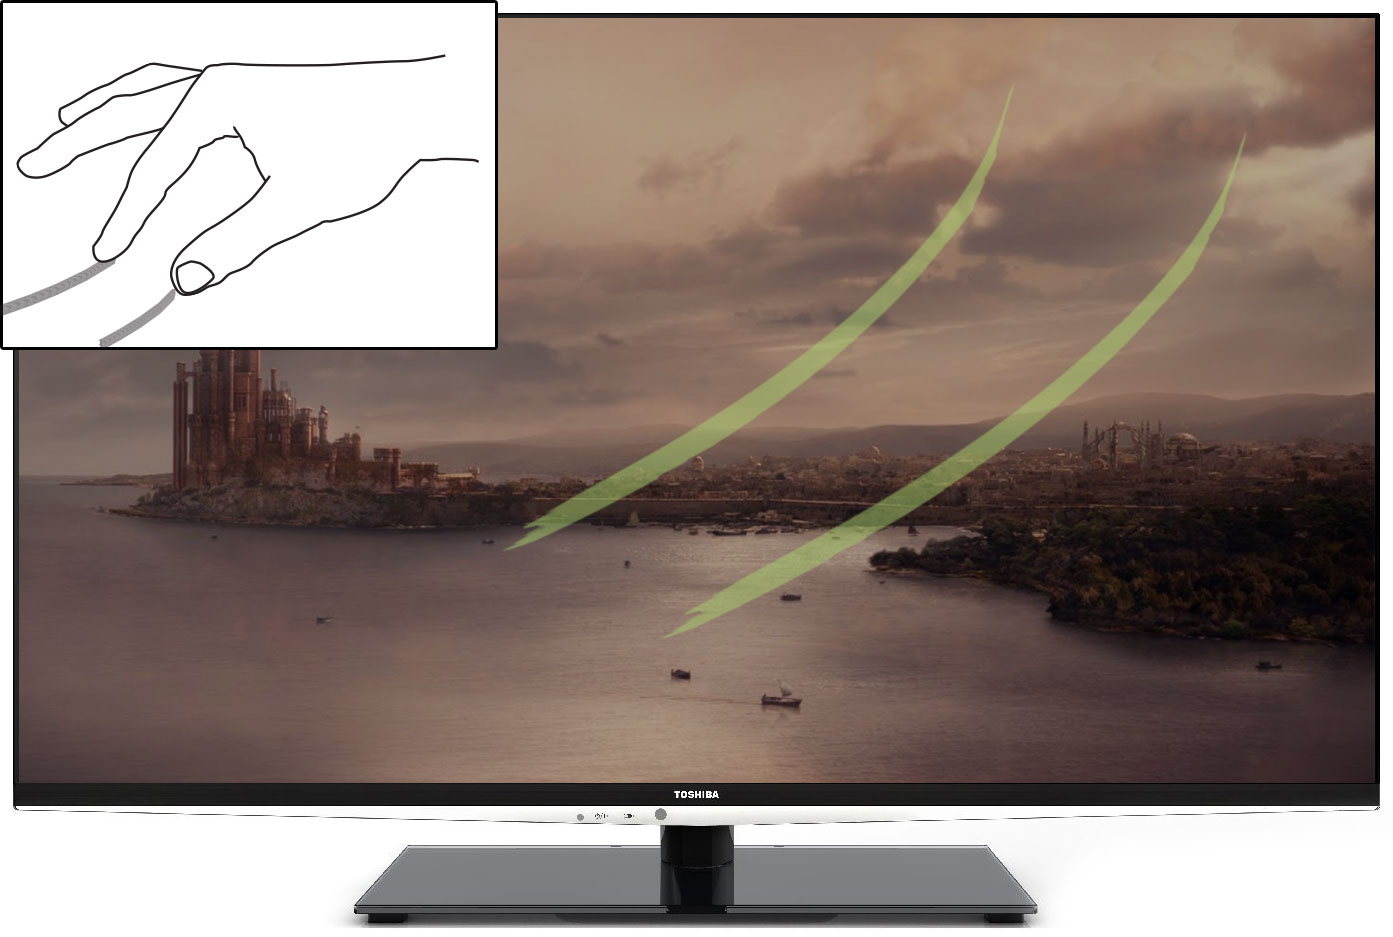
\includegraphics[width=.9\linewidth]{figures/touch/evaluation/gesture_overlay}
    \caption{The real-time overlay during touch. This ascending or descending two stroke gesture could for instance mean 'volume up' or 'down'.}
  \end{subfigure}%
  \hspace{1cm}
  \begin{subfigure}[t]{.45\textwidth}
    \centering
    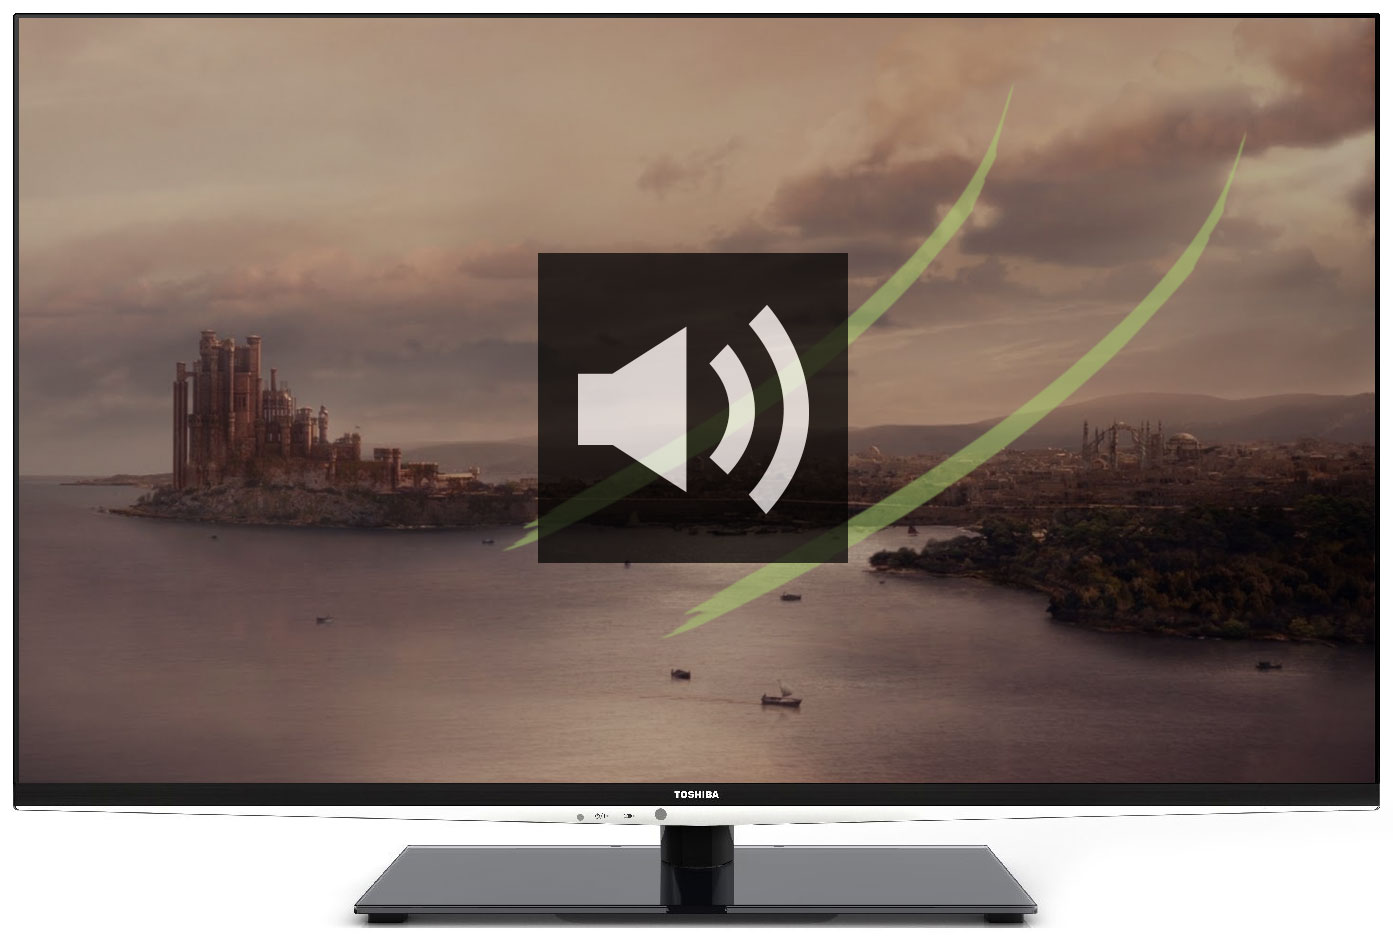
\includegraphics[width=.9\linewidth]{figures/touch/evaluation/gesture_overlay_2}
    \caption{The indication that a 'volume' action was performed.}
  \end{subfigure}
  \caption{Gesture input as an overlay for real-time feedback.}
  \label{fig:textiletouch:eval:overlay}
\end{figure}

\begin{figure}[h]
  \centering
      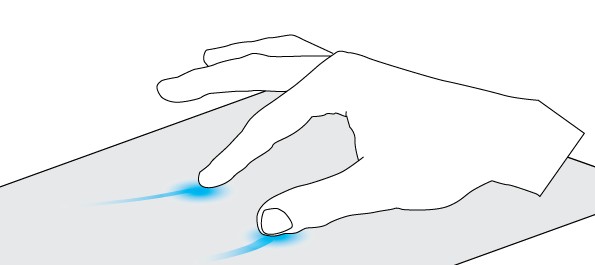
\includegraphics[width=3in]{figures/touch/evaluation/backlid_textile}
  \caption[Illumination directly beneath touch points.]
  {Illumination directly beneath touch points.}
  \label{fig:textiletouch:eval:backlighting}
\end{figure}

\begin{figure}
        \centering
        \begin{subfigure}[b]{0.45\textwidth}
                \centering
                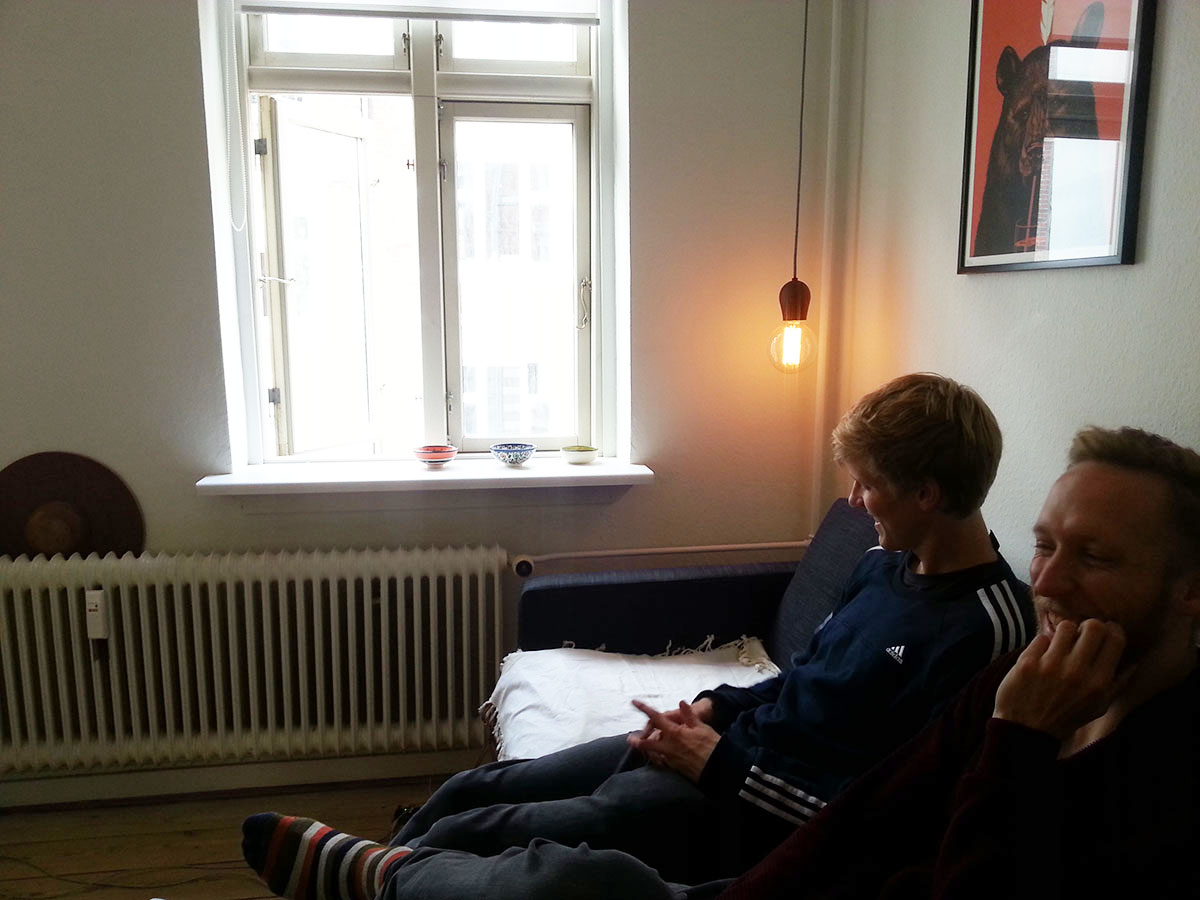
\includegraphics[width=\textwidth]{figures/touch/evaluation/sebastian/in_sofa}
                \caption{\dots}
                \label{fig:textiletouch:eval:sebastian:sofa}
        \end{subfigure}
        \begin{subfigure}[b]{0.45\textwidth}
                \centering
                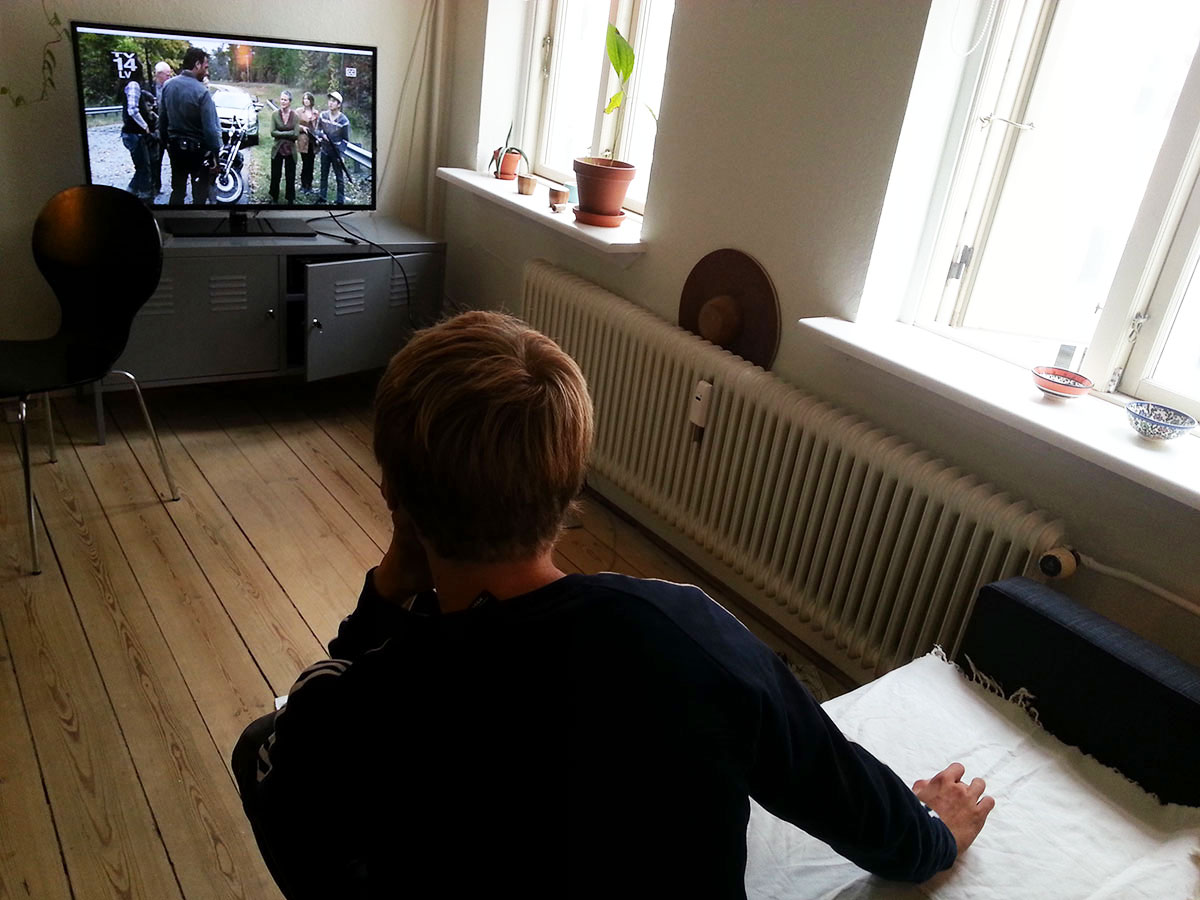
\includegraphics[width=\textwidth]{figures/touch/evaluation/sebastian/sofa_behind_seb}
                \caption{\dots}
                \label{fig:textiletouch:eval:sebastian:sofa_behind}
        \end{subfigure}

        \begin{subfigure}[b]{0.45\textwidth}
                \centering
                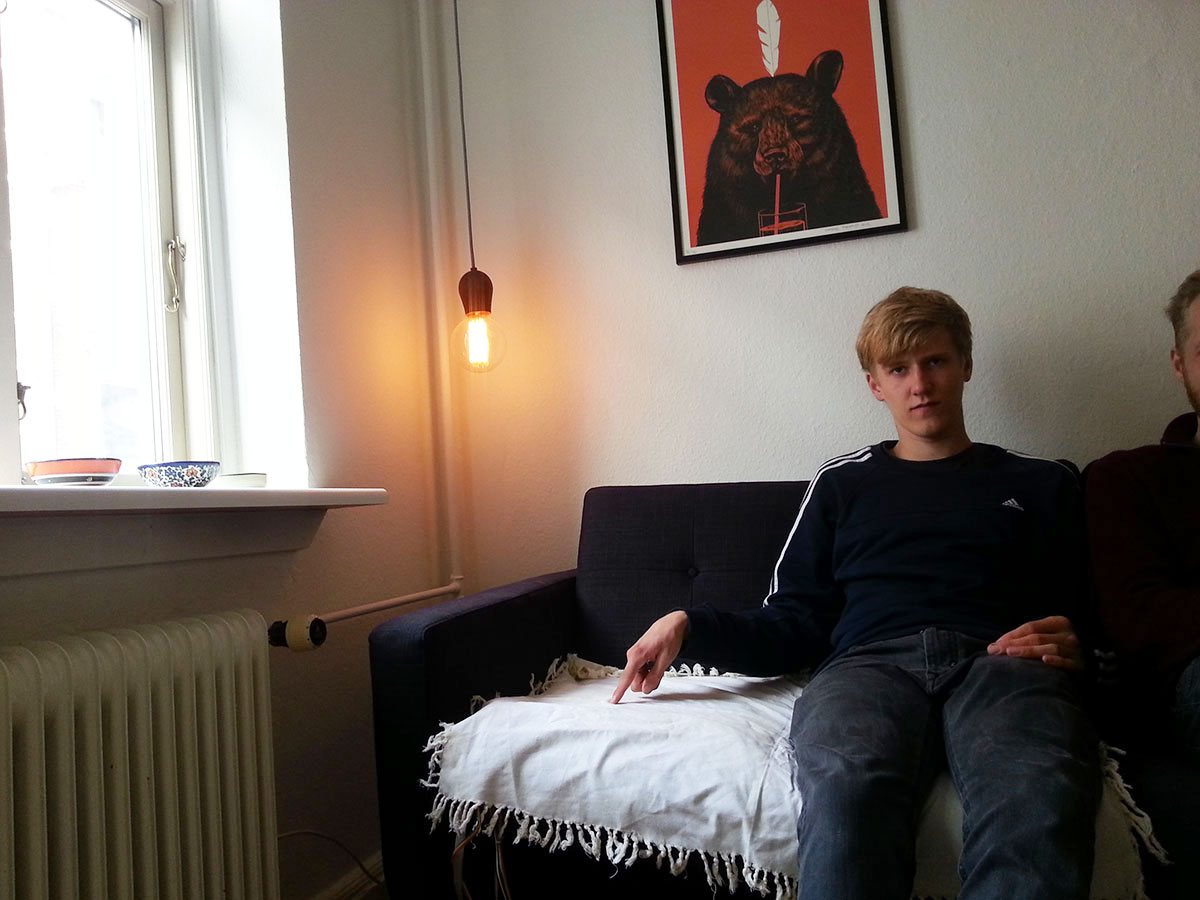
\includegraphics[width=\textwidth]{figures/touch/evaluation/sebastian/sofa_infront_seb}
                \caption{\dots}
                \label{fig:textiletouch:eval:sebastian:sofa_front}
        \end{subfigure}
        \begin{subfigure}[b]{0.45\textwidth}
                \centering
                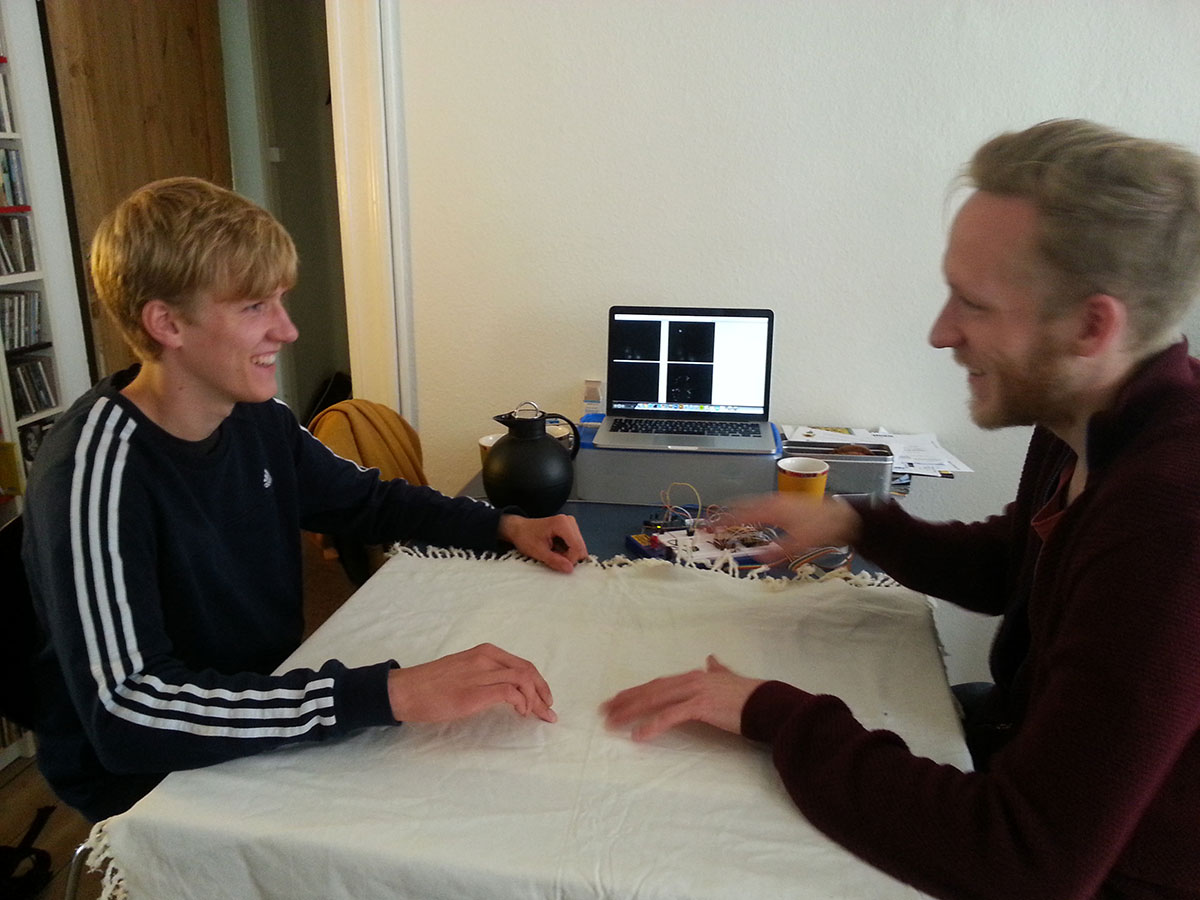
\includegraphics[width=\textwidth]{figures/touch/evaluation/sebastian/table}
                \caption{\dots}
                \label{fig:textiletouch:eval:sebastian:table}
        \end{subfigure}
        \caption{Teenager during evaluation \dots}
        \label{fig:textiletouch:eval:sebastian}
\end{figure}

\begin{figure}[h]
  \centering
      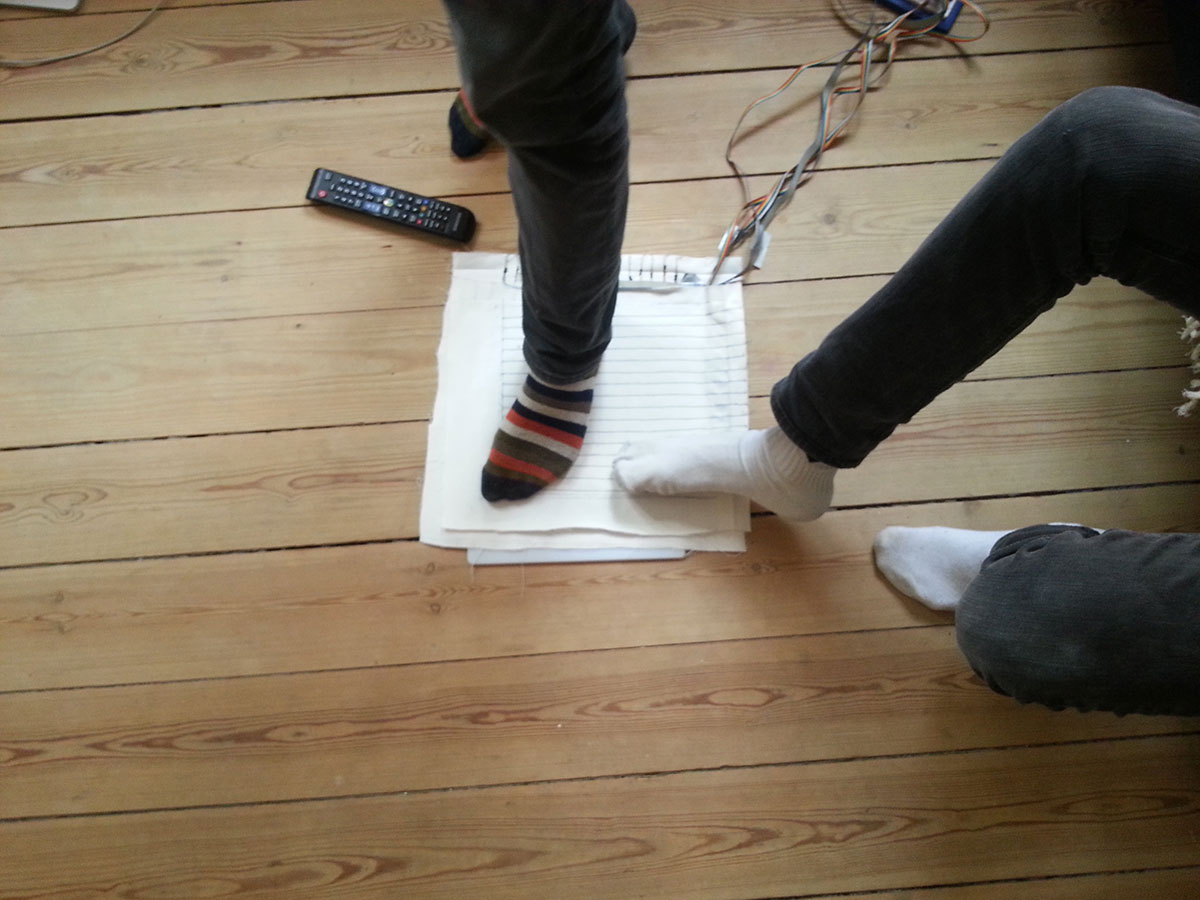
\includegraphics[width=3in]{figures/touch/evaluation/sebastian/feet}
  \caption[Feet \dots]
  {Feet \dots}
  \label{fig:textiletouch:eval:sebastian:feet}
\end{figure}


\subsection{Potentials of alternative usages}

The ideas for alternative usages were in general very different from the idea of controlling existing devices.
The ideas were more characterised by sensor data being used in situations where meaning is open to interpretation as opposed to a one-to-one mapping between input gesture and function.
For example, several ideas concerning safety and security were discussed.

% toddlers
Parents of toddlers often have floor mats for their child to lay and play on, see figure~\ref{fig:textiletouch:eval:softtiles}.
Instead of having parents checking up on their child every two minutes these mats could have touch fields embedded.
The sensor data can then be abstracted to inform parents about the activity of their child by recording pressure and movement, giving the concerned parent room to do less frequent check ups.
This is actually a very simple setup that does not require a high resolution of the sensor grid and the output required could be condensed to simple states such as, whether the toddler is on the mat and the level of movement activity.

% elders
Elderly people with a weak physic or people with Parkinson's disease have a tendency to fall over easily.
One of the approaches in reducing the consequences of a fall is to give the elders assistive devices such as wearable fall detectors which can automatically release an alarm in the event of a fall.
An alternative approach, which does not require body equipment, could be to prepare the home with sensitive impact sensitive floors or carpets.
Some may base their sense of security in a physical wearable device while others find it inconvenient, a source of irritation, or maybe even an exceedance of personal privacy. 
With safety measurements invisibly integrated into the home the sense of security may be directed towards to the scope of the home as a whole.

% handicap
Some disabled people with hindered mobility 
\blank
% Home security
During the evaluations we also discussed a scenario of home security regarding the front door of ones home.
In this scenario we imagined a blank door with no handle and no lock and thereby no need for a key.
Instead the door had an embedded grid of pressure sensors.
We came up with and enacted two different interaction styles for opening the door.
One was a variant of the pattern lock found in many Android smart phones where a set of points must be touched in the correct sequence in order for the door to unlock, see figure \todo{billede af Kaia og Gitte ved doeren 1}.
The other was based on the fact that people have unique signatures which could be used for authentication.
A person would then have to makes strokes (the signature) on the door facade to be authenticated and have the door unlock and open, see figure \todo{billede af Kaia og Gitte ved doeren 2}.

This is a good example of an ad hoc interface \emph{through invisible interfaces embedded into the physical environment}.
Knowledge of the system is a prerequisite to enter in that you are faced with a blank facade with no direct indication of how to enter.
It also confronts the raised issue of invisible interfaces and affordances by using it as an advantage in a security setting where the absence of a lock and door handle would inhibit a trespasser.
\blank
% Sleep cycle
Moving away from the topic of safety and security and to the topic of self-tracking, a movement that has gained a lot popularity in recent years with the advent of consumer gadgets, such as Fitbit\footnote{http://www.fitbit.com/}, Nike+\footnote{http://nikeplus.nike.com/plus/} and loads more. 
These gadgets let you sense just about anything concerning your body, quantifying yourself in numbers.
An example of this is sleep monitoring and optimisation, which in its simplest form only requires a smart phone next to your body in bed, but can take on more advanced forms as well with a variety of body sensors.
With a smart phone the approach is to use the built-in accelerometer to detect movement during sleep to graph the total sleep and derive whether the person is in deep sleep or light sleep.
These data can also be used to trigger the wake-up alarm at moments of light sleep within a specified time frame close to the set alarm time.

A product with the capabilities of our textile touch prototype which can infer the same kind information by the means of a pressure measurements over time, would be an interesting alternative.
Being integrated as part of a madras or a bed sheet it would be unnoticeable for a sleeping person and would not require a smart phone next to the pillow which some may be precautious about.

This application does not really fall under the category of AHIs, but it is mentioned here for the potential of a discrete and unobtrusive product as a continuation of the self-tracking movement.


\begin{figure}[h]
  \centering
      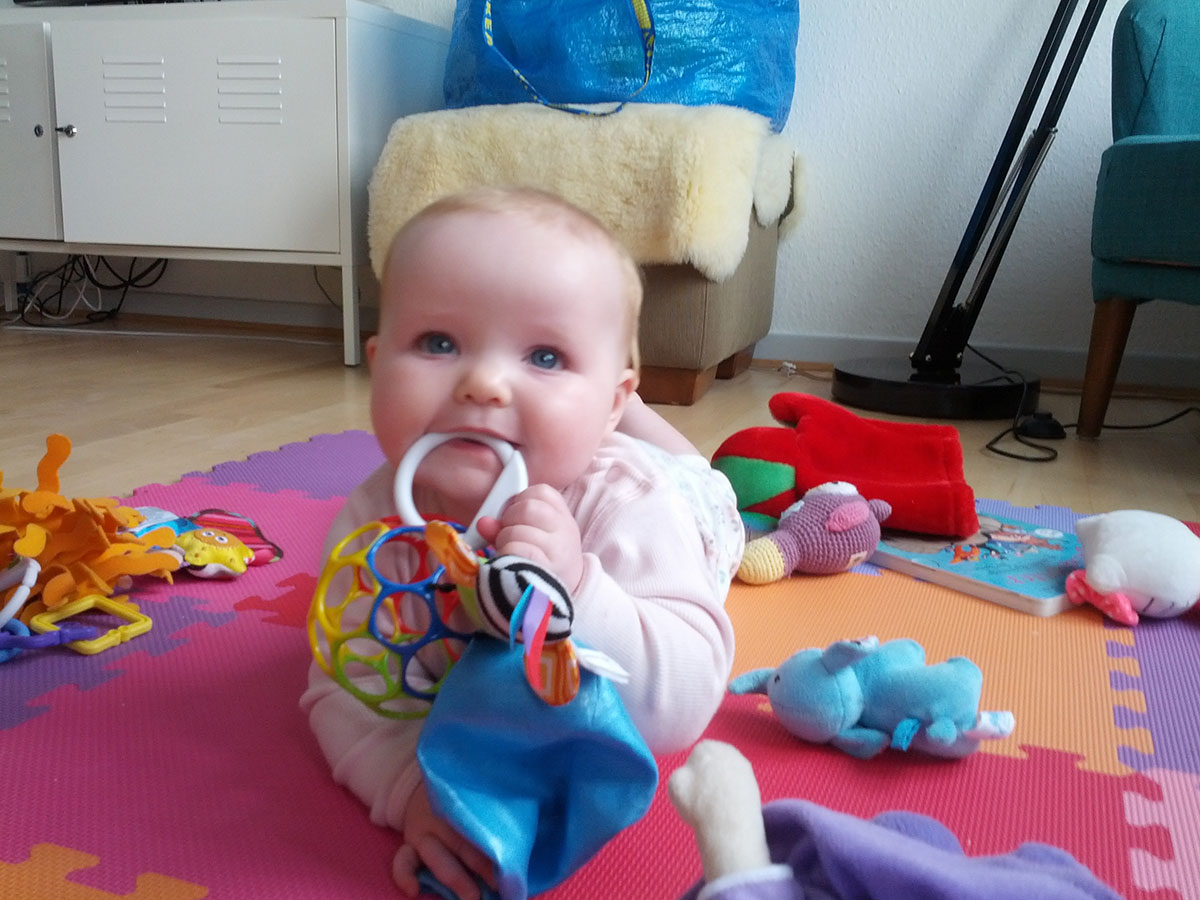
\includegraphics[width=3in]{figures/touch/evaluation/softtiles}
  \caption[Toddler on a foam floor mat with puzzle-like tiles for extensibility.]
  {Toddler on a foam floor mat.}
  \label{fig:textiletouch:eval:softtiles}
\end{figure}

\begin{verbatim}
**** Paw + Morten ****
* tegning paa overflader: "hvis danmark nu er her ... og holland her, saa ..." 
	- for at forklare ting.
* boernevaerelse - legemaatte, hvor foraeldre kan se aktivitetsniveau for 
	deres unger og dermed ikke behoever at tjekke op paa dem hele tiden.
* handikaphjem
	* vildt mange ting der skal styres
    * mobilitet er begraenset
* aeldrehjem
    * crash taeppe - folk med parkison der ofte vaelter eller lign.
        * eller alle flader
    * "hvis man ikke har noget paa kan det ikke tages" - nuvaerende situation 
		hvor aeldre faar "halsbaand" (falde-detektor) paa, som de tager af i tide og utide.
* Sikkerhed. Den usynlig noegle - man skal vide hvor man input delen er for 
	at kunne lave en "adgangsgestik".
    * Eller det, at mennesker har en unik "haandskrift" der kan anvendes 
		paa touch overfladen.
    * doermaatte
\end{verbatim}

\subsection{Future work}
\label{ch:textiletouch:futurework}

There are several points about the prototype that are candidates for future work.

% Multitouch
On the technical side there is room for improvement.
As the technology allows for multi-touch input it would be a great improvement for the user experience.
Multi-touch provides a much richer interaction style \todo{reference?} compared to single-touch and has become a standard in modern smart phone displays and laptop touchpads, most notably for scrolling, zooming and rotation.
The gesture recognition framework used for the prototype, \$P, will work just fine with multi-touch and will not require further adjustment as the method of input is totally decoupled from the recognition framework. \todo{though gestures or symbols are not the same as real-time gestures on a mouse-pad such as zooming}
Instead it is our peak detection algorithms that need to be reimplemented and take multiple peaks in to account.
Figure~\todo{ref} shows a frame of input where several peaks made by finger inputs are detected. \todo{provide reason for not implementing multi-touch in the firstplace?}

As can be seen in the figure every peak is surrounded by some noise created by finger pressure propagating away from the peak spot.
It should be noted that we do not consider values in the immediate proximity of a peak to be noise as we use these values to make interpolation and thereby scale the resolution by a factor a 10.
We have already taken steps to reduce this by implementing a simple averaging filter in the software 
where a sample is an average of \emph{x} previous samples.
There are also steps to be taken on the hardware side where a noise filter could reduce the signal-to-noise ratio before entering the software part.

\todo{ting der er belyst fra evaluering \dots}

\begin{verbatim}
dette er ikke faerdig prototype - snakke om forskellige retninger
Real-world implementation - e.g. a whole sofa, wall paper?
\end{verbatim}

